\documentclass[12pt]{article}
\usepackage{romannum}
\usepackage{graphicx}
\usepackage{float}
\title{Time Series Project}
\author{Simone Quadrelli 938667}
\newpage
\begin{document}
\pagenumbering{gobble}
\maketitle
\newpage
\tableofcontents
\pagenumbering{roman}
\newpage
\section{Introduction}
\pagenumbering{arabic}
The project concerns the analysis of the relationship between one month interest rate and one year interest rate, respectively referred as short-term interest rate and long-term interest rate, of riskless discount bonds. The dataset analyzed consists in the interest rates measured by the Federal Reserve between January 1986 and December 2008. The information prior to January 1986 are known but not used due to the policy of the Federal Reserve.
\\Central banks influence long-term interest rates by modifying  short-term interest rates. Therefore it is crucial to understand if the two interest rate are cointegrated, meaning that the short-term interest rates really influence long-term interest rates.
\\Section \ref{sec:1} provides a brief overview of the data and the unit root tests, while section \ref{sec:2} concerns the cointegration of the series. Section \ref{sec:3} concerns the testing of the expectation hypothesis under rational expectations.
\section{Unit root test} \label{sec:1}
The data analyzed are continuously compounded interest rates on riskless discount bonds with one month maturity ($m1$ series) and one year maturity ($y1$ series).
\\To understand whether the process representing m1 (one month maturity) is stationary or not, a unit root test is required. Augmented Dickey-Fuller test (the unit root test used) is sensitive to the possible presence of an intercept. Indeed, if the unit root is present then  the estimation $ m1_t =  \beta m1_{t-1}$ has the same probability not to reject the null hypothesis as $ m1_t = \alpha + \beta m1_{t-1}$. On the contrary, if there is not a unit root and the intercept $\alpha =  0$ is less easy to reject the null hypothesis in $ m1_t = \alpha + \beta m1_{t-1}$; if $\alpha \neq 0$ then $ m1_t =  \beta m1_{t-1}$ becomes inconsistent. Thus, if it is not known for sure that there is an intercept, the estimation $ m1_t = \alpha + \beta m1_{t-1}$ should be preferred. Since it is not reasonable to exclude the presence of an intercept as Figure \ref{fig:dataplot} hints, the regression $ m1_t = \alpha + \beta m1_{t-1}$ should fit the data better than  $ m1_t =  \beta m1_{t-1}$.
\begin{figure}[H]
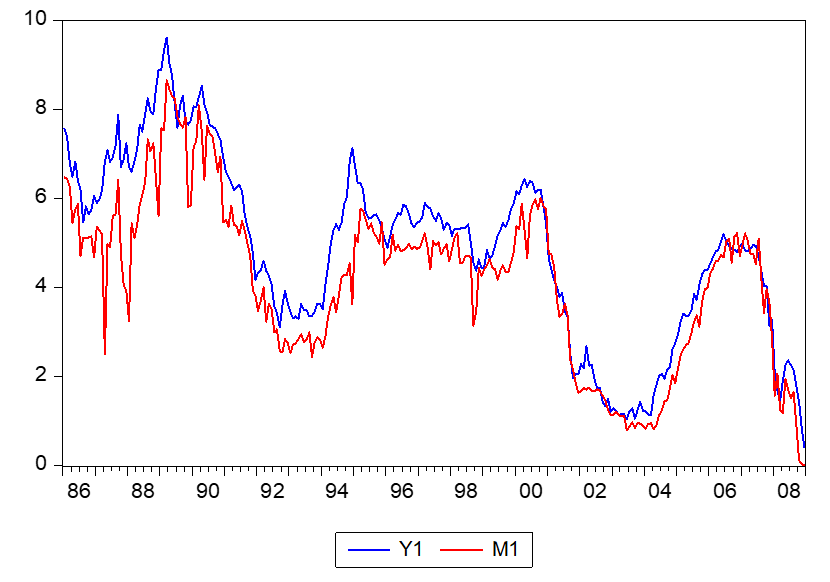
\includegraphics[scale=1]{plot.PNG} 
\caption{Term structure of one month interest rate and one year interest rate. Plot of one month interest rate in red, plot of one year interest rate in blue. \label{fig:dataplot}}
\end{figure}
\noindent As the unit root test in Figure \ref{fig:m1unitroot} shows, the hypothesis that m1 has a unit root is not rejected, indeed its t-Statistic value (-1.4718930) is greater than the 5\% critical values (-2.871806) of the Augmented Dickey-Fuller test. Therefore it is possible to state that $m1 \in I(1)$ (i.e $m1$ series is integrated of order one). 
\begin{figure}[H]
\centering
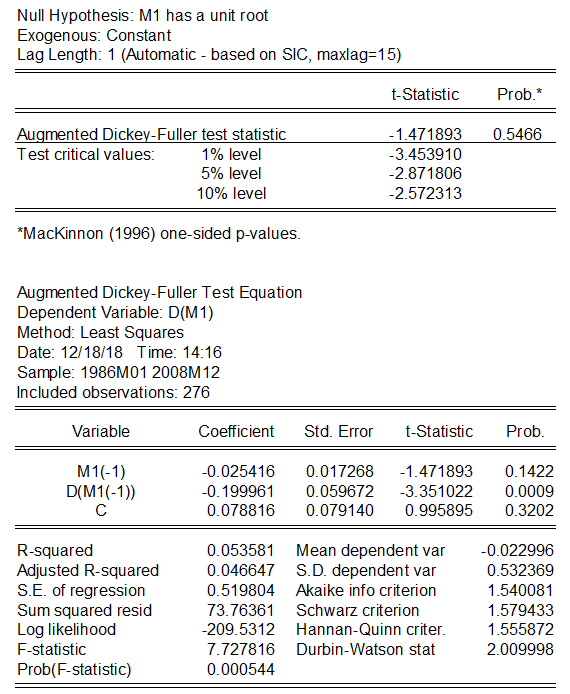
\includegraphics[scale=1]{m1_unit_root_test.PNG} 
\caption{Unit root test concerning one month interest rate \label{fig:m1unitroot} }
\end{figure}
\noindent Moreover, the same reasoning holds for $y1$ (one year maturity) series. It is reasonable to believe that y1 series has an intercept because the mean of the interest rate is positive. Therefore the regression $ y1_t = \alpha + \beta y1_{t-1}$ should fit the data better than  $ y1_t =  \beta y1_{t-1}$. As Figure \ref{fig:y1unitroot} suggests, the hypothesis that y1 has a unit root is accepted, indeed its t-Statistic value (-1.4718930) is greater than the 5\% critical values (-2.871806) of the Augmented Dickey-Fuller test.  Therefore it is possible to state that $y1 \in I(1)$ (i.e  $y1$ series is integrated of order one).

\begin{figure}[H]
\centering
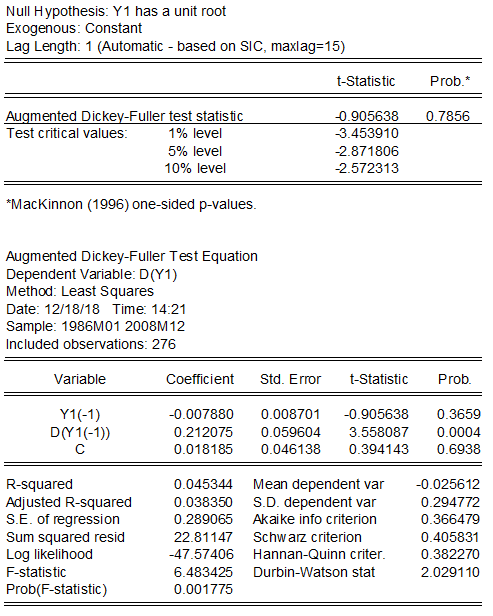
\includegraphics[scale=1.2]{y1_unit_root_test.PNG} 
\caption{Unit root test concerning one year interest rate \label{fig:y1unitroot} }
\end{figure}

\section{Cointegration test} \label{sec:2}
If the series $y1$ depends on the series $m1$, then a monetary  policy that influences the short-term interest rate can, in turn, influence the long-term interest rate. To understand if that is true, it is possible to run a cointegration test on the series. Two series are said to be cointegrated if the residuals $r_t$ of $y1_t -\beta m1_t$ \footnote{$\beta = 1$} are integrated of order zero ($r_t \in I(0)$). The difference between the yearly interest rate $y1_t$ or $i_{12,t}$ and the monthly interest rate $m1_t$ or $i_{12,t}$ is called \textit{term spread} $S^{(12,1)}_t = i_{12,t} - i_{1,t}$.  As Figure \ref{fig:cointegrationtest} shows, the null hypothesis that the two series are not cointegrated is rejected, therefore it is possible to state that the series are cointegrated and that $y1$ depends on $m1$.
\begin{figure}[H]
\centering
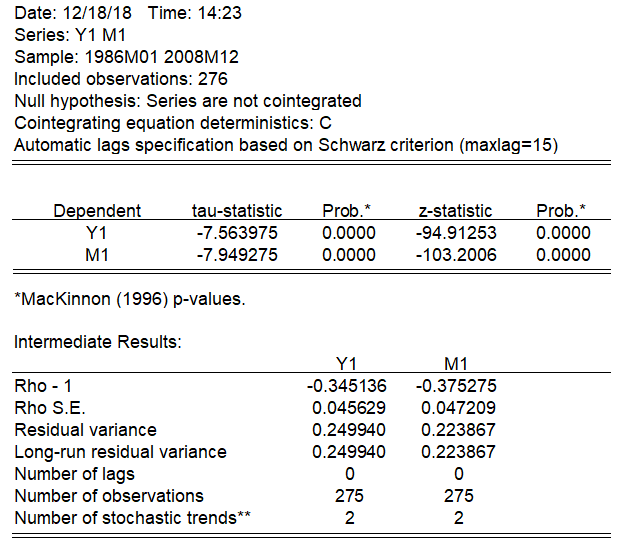
\includegraphics[scale=1]{cointegration_test.PNG} 
\caption{Cointegration Test \label{fig:cointegrationtest} }
\end{figure}
\noindent Moreover, it is possible to estimate the coefficient $ \beta $ in the regression  $y1_t = \alpha + \beta m1_t$. The estimation $\hat{\beta}$ of $\beta$ is expected to be approximately $1$, by the definition of cointegration. The parameter $\hat{\beta}$ corresponds to the value C(2) in Figure \ref{fig:betaestim} and indeed $\hat{\beta} \approx 1$.
\begin{figure}[H]
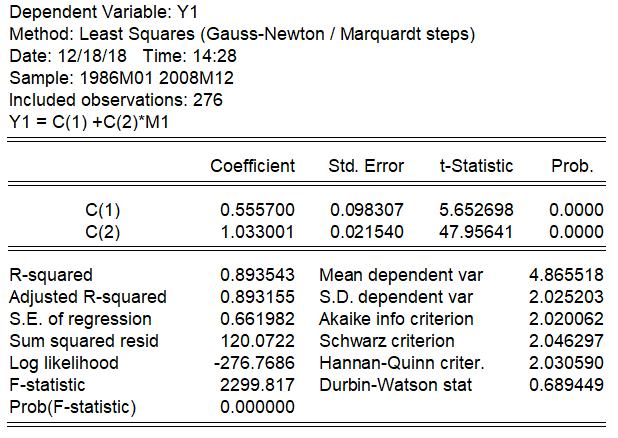
\includegraphics[scale=1]{beta_estimation.PNG} 
\centering
\caption{Estimation of $\beta$ \label{fig:betaestim}}
\end{figure}
\noindent To guarantee the cointegration, it is also possible to exploit the definition by testing the presence of a unit root in the residuals of $y1_t- \hat{\beta}m1_t = S^{(12,1)}$. Indeed, by definition, two series are cointegrated if their residuals are integrated of order zero, so it is possible to run a unit root test on the residuals. The test denies the possibility of a unit root (Figure  \ref{fig:unitroottest}). Therefore it is possible to state that the $y1$ and $m1$ are cointegrated.
\begin{figure} [H]
\centering
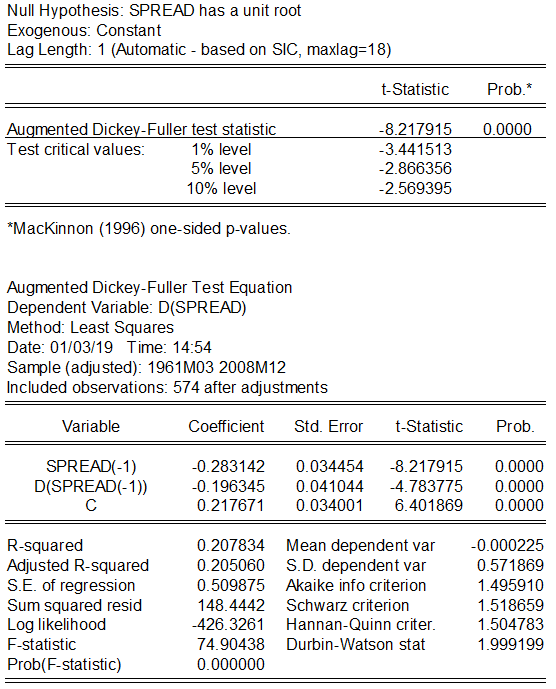
\includegraphics[scale=1]{unit_root_spread_test.PNG} 
\caption{Unit root test on the term spread $S^{(12,1)}$ \label{fig:unitroottest}}
\end{figure}

\section{The expectations hypothesis under rational expectations} \label{sec:3}
It is interesting to understand if the expectations hypothesis holds under rational expectations. The expectation hypothesis states that the economic agents maximize the expected profits of their investments. They can invest or borrow money with long-term contact or with a sequence of short-term contracts, considering also possible term premia.
As a start, it is convenient to suppose there are no term premia, so interest rate at time 2 is 
\begin{equation}
i_{2,t} = \frac{1}{2}(i_{1,t}+E_t(i_{1,t+1})).
\end{equation}
\\The model can be expanded to take in account possible exogenous events, adding independent and identically distributed shocks $e_{n,t}$ under two restrictions:
\begin{itemize}
\item $E_t(e_{n,t})  = 0$ \footnote{$E_t$ means the expected value of $ e_{n,t} $ at time $t$}
\item $Var(e_{n,t})= \sigma^2$
\end{itemize}
Generalizing the reasoning concerning the spread to a generic time n,
\begin{equation}
i_{n,t} = \frac{1}{n}(i_{1,t} + \sum_{l=2}^nE_t(i_{n,t+l}))
\end{equation} holds.
\\Since Rational Expectation (RE) is assumed to hold, it is possible to define the expected value of the interest rate as
\begin{equation} \label{eq1}
E_t(i_{n,t+k})= i_{n,t+k} + e_{n,t+k},
\end{equation} where $E_t( e_{n,t+k}) = 0 \; \forall t,k \in N$.
\\When substituting in the expectation (Eq. \ref{eq1}) into
$i_{n,t} = \frac{1}{n}(i_{1,t} + \sum_{l=2}^nE_t(i_{n,t+l}))$, it becomes
\begin{equation}
i_{n,t} = \frac{1}{n} \sum_{l=1}^{n}i_{n,t} + \frac{1}{n}\sum_{l=2}^{n-1}\epsilon_{l,t+n} + e_{n,t}.
\end{equation}
\\Let 
\begin{equation}
\eta_{t+n} = \frac{1}{n}(\sum_{l=2}^{n-1}\epsilon_{l,t+n}) + e_{n,t},
\end{equation}
\\now it is possible to rewrite $i_{n,t}$ as
\begin{equation}
i_{n,t}= T_n + i_{1,t} + \sum_{l=1}^{n-1}\frac{n-l}{n}\Delta i_{1,t+l}+\eta_{n+t},
\end{equation} when a term premia $T_n$ is added.
\\Rearranging the terms it is possible to obtain 
\begin{equation}
\sum_{l=1}^{n-1}\frac{n-l}{n}\Delta i_{1,t+l} = -T_n + (i_{n,t}-i_{1,t}) - \eta_{t+n})
\end{equation} that can be estimated as
\begin{equation} \label{eq:2}
\sum_{l=1}^{n-1}\frac{n-l}{n}\Delta i_{1,t+l} = \alpha_s + \beta_s S^{(n,1)}_t +u_{t+n}.
\end{equation}
Since the analysis concerns one year interest rate and one month interest rates Eq. \ref{eq:2} becomes
\begin{equation} 
\sum_{l=1}^{n-1}\frac{n-l}{n}\Delta i_{1,t+l} = \alpha_s + \beta_s S^{(12,1)}_t +u_{t+n}.
\end{equation}
\\It is worth noticing that by definition $u_{t+n}$ should be independent and identically distributed, but in the dataset the independence is not granted as Figure \ref{fig:testonresiduals} shows.
\begin{figure}[H]
\centering
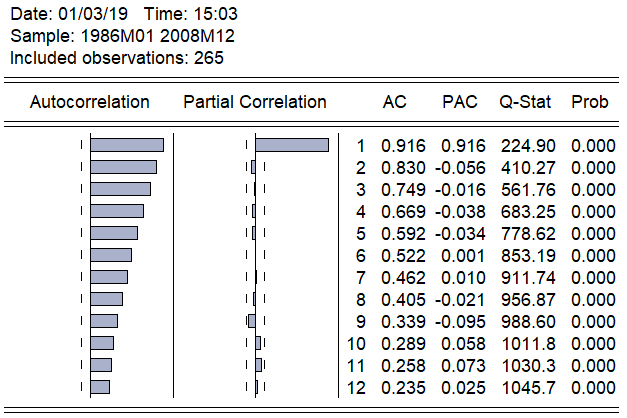
\includegraphics[scale=1]{test_on_residuals.PNG} 
\caption{Wald test on $u_{t+n}$ \label{fig:testonresiduals}}
\end{figure}
\noindent Since $u_{t+n}$ are not independent we use an appropriate method of estimation (Figure \ref{fig:expectationhypothesis}) to obtain $\sum_{l=1}^{n-1}\frac{n-l}{n}\Delta i_{1,t+l} = \alpha_s + \beta_s S^{(12,1)}_t +u_{t+n}$.
\begin{figure}[H]
\centering
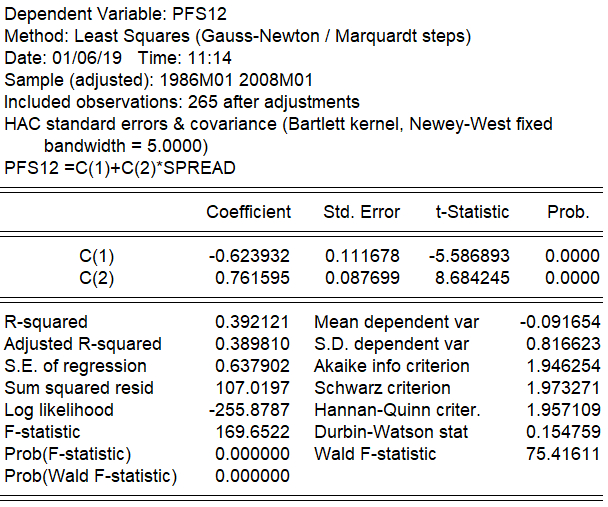
\includegraphics[scale=1]{expectation_hypothesis.PNG} 
\caption{Estimation of $\alpha_s + \beta_s S^{(n,1)}_t +u_{t+n}$ \label{fig:expectationhypothesis}}
\end{figure}
\noindent The expectation hypothesis and the pure expectation hypothesis hold at least if $\beta_s = 1$.
\begin{figure}[H]
\centering
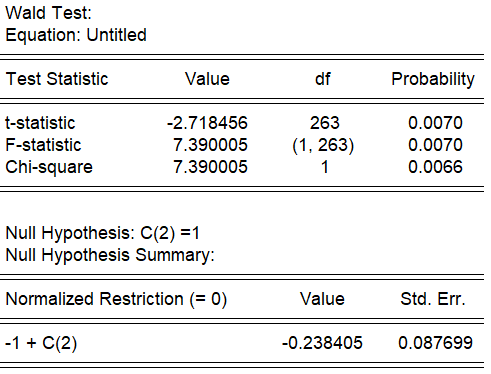
\includegraphics[scale=1]{beta_hypothesis_test.PNG} 
\caption{Test if $ \beta_s=1$\label{fig:betahypothesistest}}
\end{figure}
\noindent Given the coefficients $\alpha_s$ and $\beta_s$, it is possible to test whether coefficient $\beta_s = 1$ (corresponding to c(2) in Figure \ref{fig:betahypothesistest}) or not. As Figure \ref{fig:betahypothesistest} show, it is possible to state that the null hypothesis $\beta_s=1$ is rejected, therefore the pure expectation hypothesis and expectation hypothesis under rational expectation do not hold.

\section{Conclusions} \label{sec:4}
The analysis show that the series representing respectively continuously compounded one month interest  rate ($m1$) and one year interest rate ($y1$) on discount bonds are both integrated of order one. 
\\ It is also possible to state that $y1$ and $m1$ are cointegrated meaning that changes in $m1$ modify $y1$, so the central bank can influence long-run interest rates by modifying short-term interest rates. This relationship implies that the term spread provides a useful information to foretell the interest rate dynamic, nevertheless the expectations hypothesis under rational expectations is rejected. 
\end{document}
